\documentclass[milestone1.tex]{subfiles} 
\begin{document}

%% ----------------------------------------------
% Section Experiments
%% ----------------------------------------------
\section{Experiments}


\subsection{Microbenchmarks}

The goal of the microbenchmarks is to understand single components and units.

\subsubsection{Send Message}

The time to send a message has been measured:




\subsection{Test Protocol}

The whole test protocol can be found on the Testmasters\footnote{https://testmaster-asl-eth.renuo.ch and https://testmaster2-asl-eth.renuo.ch}. Additionally, a short summary of the test protocol can be found in the directory \textit{ethz-asl-mlmq/doc/test\_protocol}.

\subsection{Testload}
To generate test load for the messaging system a mixture of different types of clients will be chosen. This section describes these clients.

\subsubsection{OneWayClient}
As stated in the project description each OneWayClient sends an initial message to an arbitrary other one. Having it's initial message sent they periodically check their personal queue for incoming messages. If there is one the message is dequeued and forwarded to a random receipient.

Sent messages contain a simple counter which is increased each time a message is relayed.

\subsubsection{PairedClient}
PairedClient's always come in pairs. They keep on sending requests and responses to each other. At start it is determined which client is the requesting client and which is the responding client.

\subsubsection{PublicQueueProducer}
This kind of client writes the same message again and again to a public queue.

\subsubsection{PublicQueueConsumer}
This kind of client tries to read messages at a constant rate from a public queue.

\subsection{2 Hour Test}


% for each experiment
%- why are we doing this experiment
%- hypothesis
%- experiment setup (parameters)
%- plots of the result
%- describe the plot
%- explain the plot/experiment

To verify that the system runs stable over a long period of time an experiment is performed which puts a constant load onto the system for 2 hours.\\

During the project, the system evolved and thus some test runs were invalidated in this process. Here, the final two 2h test runs are presented. The other 2h test runs can be found and analysed on the Testmaster\footnote{https://testmaster-asl-eth.renuo.ch/}.\\

\paragraph{Experiment setup}
The experiment is performed on the Amazon cloud with with constant load. For the setup configuration, the project specifications were used specifications (80 clients).\\

\begin{tabular}{|l|l|}
\hline 
Parameter & Value \\
\hline 
Amazon instance type and availiblity zone for the database & m1.medium, eu-west-1a \\ 
Amazon instance type and availiblity zone for the middlewares & m1.small, eu-west-1a \\ 
Amazon instance type and availiblity zone for the clients & m1.small, eu-west-1a \\ 
Number of middlewares & 2 \\ 
OneWayClient & 1x30 (machines x jvms) \\ 
PairedClient & 1x16 (machines x jvms) \\ 
PublicQueueConsumeClient / PublicQueueProduceClient & 2x15 (machines x jvms) \\
Middlware & 2x3 (machines x jvms) \\ 
Client message send interval (TODO: think time?) & 10ms \\
\hline 
\end{tabular}

\paragraph{Hypothesis}
Since the system will not be saturated we expect no changes over time concerning response time and throughput. The mixture of clients generating load is chosen such that there is a constant number of messages in the system. Increased SQL query execution time should not be observable.

\paragraph{Results}
There were multiple 2h tests performed. The final two 2h tests are the ones with id 174 \footnote{https://testmaster-asl-eth.renuo.ch/test\_runs/174} and 176 \footnote{https://testmaster-asl-eth.renuo.ch/test\_runs/176}. Both run stable and generated the following plots:

TODO: insert plots

\paragraph{Interpretation}
The final test runs (174 and 176) run as expected in the hypothesis.

%% -------------------------------------------
%% 2^k Experiment
%% -------------------------------------------
\subsection{$2^k$ Experiment}
In order to determine the influence of a number of primary factors on to the system it was decided to do a $2^k$ analysis on several factors described in the following section.

For each feature level an experiment of 30 minutes is performed where clients perform 100 actions (send and receive message) per second.

\subsubsection{Factors and Levels}

\paragraph{Number of Clients}
The number of simultaneously connected clients is varied between 8 and 30. There is a mix of different clients which produce slightly different types of load.

\begin{tabular}{|l|c|c|}
\hline 
 & Lower Level & Upper Level \\ 
\hline 
OneWayClient & 16 & 8  \\ 
\hline 
PairedClient & 8 & 4 \\ 
\hline 
PublicQueueConsumer & 4 & 2 \\ 
\hline 
PublicQueueProducer & 2 & 1 \\ 
\hline 
\textbf{Total}  & \textbf{30} & \textbf{15} \\
\hline 
\end{tabular} 

\paragraph{Number of brokers}

The number of middleware components is varied between 4 and 8. For both levels the number of Amazon instances used is 2.

\paragraph{Number of workers}

The number of worker threads a single middle ware instance has is varied between 4 and 8

\paragraph{Number of Database Connections}

The number of concurrent database connection a single middle ware instance has is varied between 4 and 8


\subsubsection{Hypothesis}

The response time should not be majorly affected by these chosen parameters. Since the system is not under much load only small changes concerning the response time should be observable.

However the number of requests processes should vary. The main feature which obviously affects number of requests is the number of connected clients sending messages. Other minor variations will reveal bottle necks in the system.

\subsubsection{Measurement Results}
The following table shows median time taken and number of requests processed for all different feature levels.\\

\begin{figure}[H]
	\begin{center}
	
\begin{tabular}{cccccccc}
\rot{Clients C} & 
\rot{Brokers B} & 
\rot{Workers W} & 
\rot{Connections D} & 
\rot{TestRun Id} & 
\rot{Median Processing time [ms] PT} & 
\rot{\# of Processed Requests RC} \\
\hline 
15 & 4 & 4 & 4 & 2003 & \numprint{6.80} & \numprint{1996478} \\ 
\hline 
15 & 4 & 4 & 8 & 173 & \numprint{7.46} & \numprint{1806665} \\ 
\hline 
15 & 4 & 8 & 4 & 2007 & \numprint{6.87} & \numprint{2062704} \\ 
\hline 
15 & 4 & 8 & 8 & 2008 & \numprint{7.21}  & \numprint{2060655} \\ 
\hline 
15 & 8 & 4 & 4 & 2009 & \numprint{5.11} & \numprint{1385552} \\ 
\hline 
15 & 8 & 4 & 8 & 2004 & \numprint{7.55} & \numprint{1910840} \\ 
\hline 
15 & 8 & 8 & 4 & 2005 & \numprint{5.90} & \numprint{1975889} \\ 
\hline 
15 & 8 & 8 & 8 & 2006 & \numprint{7.60} & \numprint{1920835} \\ 
\hline 
30 & 4 & 4 & 4 & 159 & \numprint{14.08} & \numprint{2488948} \\ 
\hline 
30 & 4 & 4 & 8 & 160 & \numprint{12.80} & \numprint{2451248} \\ 
\hline 
30 & 4 & 8 & 4 & 161 & \numprint{13.42} & \numprint{2428769} \\ 
\hline 
30 & 4 & 8 & 8 & 162 & \numprint{13.97} & \numprint{2511260}  \\ 
\hline 
30 & 8 & 4 & 4 & 163 & \numprint{12.43} & \numprint{2329883} \\ 
\hline 
30 & 8 & 4 & 8 & 164 & \numprint{14.85} & \numprint{2110459} \\ 
\hline 
30 & 8 & 8 & 4 & 165 & \numprint{12.88} & \numprint{2266237} \\ 
\hline 
30 & 8 & 8 & 8 & 166 & \numprint{15.05} & \numprint{2166303}  \\ 
\hline 

\end{tabular} 
\end{center}
\caption{$2^4$ factorial test measurements}
\label{fig:2kfactorialmeasurement}
\end{figure}

\paragraph{Signs}

For the $2^k$ test the following signs are assigned to feature leavels:\\


\begin{figure}[H]
	\begin{center}
\begin{tabular}{|l|c|c|}
\hline 
Feature & +1 Level & -1 Level \\ 
\hline 
Number of Clients \textbf{C} & 30 & 15 \\ 
\hline 
Number of Brokers \textbf{B} & 8 & 4 \\ 
\hline 
Number of Workers \textbf{W} & 8 & 4 \\ 
\hline 
Number of Database Connections \textbf{D} & 8 & 4 \\ 
\hline 
\end{tabular} 
\end{center}
\caption{Feature Level Signs}
\end{figure}

This leads to the following sign table.


\begin{figure}[H]
	\begin{center}
\begin{tabular}{ccccccccccccccccc}
\hline 
 & I &	c&	b&	w&	d&	cb&	cw&	cd&	bw&	bd&	wd&	bwd&	cwd&	cbd&	cbw&	cbwd \\
\hline 
&1&	-1&	-1&	-1&	-1&	1&	1&	1&	1&	1&	1&	-1&	-1&	-1&	-1&	1 \\
&1&	-1&	-1&	-1&	1&	1&	1&	-1&	1&	-1&	-1&	1&	1&	1&	-1&	-1 \\
&1&	-1&	-1&	1&	-1&	1&	-1&	1&	-1&	1&	-1&	1&	1&	-1&	1&	-1 \\
&1&	-1&	-1&	1&	1&	1&	-1&	-1&	-1&	-1&	1&	-1&	-1&	1&	1&	1 \\
&1&	-1&	1&	-1&	-1&	-1&	1&	1&	-1&	-1&	1&	1&	-1&	1&	1&	-1 \\
&1&	-1&	1&	-1&	1&	-1&	1&	-1&	-1&	1&	-1&	-1&	1&	-1&	1&	1 \\
&1&	-1&	1&	1&	-1&	-1&	-1&	1&	1&	-1&	-1&	-1&	1&	1&	-1&	1 \\
&1&	-1&	1&	1&	1&	-1&	-1&	-1&	1&	1&	1&	1&	-1&	-1&	-1&	-1 \\
&1&	1&	-1&	-1&	-1&	-1&	-1&	-1&	1&	1&	1&	-1&	1&	1&	1&	-1 \\
&1&	1&	-1&	-1&	1&	-1&	-1&	1&	1&	-1&	-1&	1&	-1&	-1&	1&	1 \\
&1&	1&	-1&	1&	-1&	-1&	1&	-1&	-1&	1&	-1&	1&	-1&	1&	-1&	1 \\
&1&	1&	-1&	1&	1&	-1&	1&	1&	-1&	-1&	1&	-1&	1&	-1&	-1&	-1 \\
&1&	1&	1&	-1&	-1&	1&	-1&	-1&	-1&	-1&	1&	1&	1&	-1&	-1&	1 \\
&1&	1&	1&	-1&	1&	1&	-1&	1&	-1&	1&	-1&	-1&	-1&	1&	-1&	-1 \\
&1&	1&	1&	1&	-1&	1&	1&	-1&	1&	-1&	-1&	-1&	-1&	-1&	1&	-1 \\
&1&	1&	1&	1&	1&	1&	1&	1&	1&	1&	1&	1&	1&	1&	1&	1 \\

\hline 

\rot[90]{\textbf{Weights PT~}} & 
\rot[90]{\textbf{10.24}} &	
\rot[90]{\textbf{3.43}} &	
\rot[90]{-0.07} &	
\rot[90]{0.11} &	
\rot[90]{\textbf{0.56}} &	
\rot[90]{0.19} &	
\rot[90]{0.03} &	
\rot[90]{-0.08} &	
\rot[90]{0.07} &	
\rot[90]{\textbf{0.52}} &	
\rot[90]{0.03} &	
\rot[90]{-0.15} &	
\rot[90]{0.16} &	
\rot[90]{0.13} &	
\rot[90]{-0.05} &	
\rot[90]{-0.10} \\
\hline 

\rot[90]{\textbf{Weights RC~}} & 
\rot[90]{\numprint{2117045}} &      
\rot[90]{\numprint{227093}} & 
\rot[90]{\numprint{-108795}} & 
\rot[90]{\numprint{57036}} & 
\rot[90]{\numprint{237}} & 
\rot[90]{\numprint{-17122}} & 
\rot[90]{\numprint{-58032}} & 
\rot[90]{\numprint{-34558}} & 
\rot[90]{\numprint{17030}} & 
\rot[90]{\numprint{18621}} & 
\rot[90]{\numprint{-9556}} & 
\rot[90]{\numprint{-48050}} & 
\rot[90]{\numprint{39516}} & 
\rot[90]{\numprint{-64140}} & 
\rot[90]{\numprint{-17984}} & 
\rot[90]{\numprint{47962}} \\


\end{tabular}
\end{center}
\caption{$2^4$ factorial test result}
\label{fig:2kfactorialresults}
\end{figure}

\subsubsection{Interpretation}
It was chosen to ignore the calculated weights for processed request counts RC because big values are more difficult to read and because both observed values correlate quite well (what is shown in \ref{fig:2kmeasuredresults}.

\begin{figure}[H]
	\begin{center}
    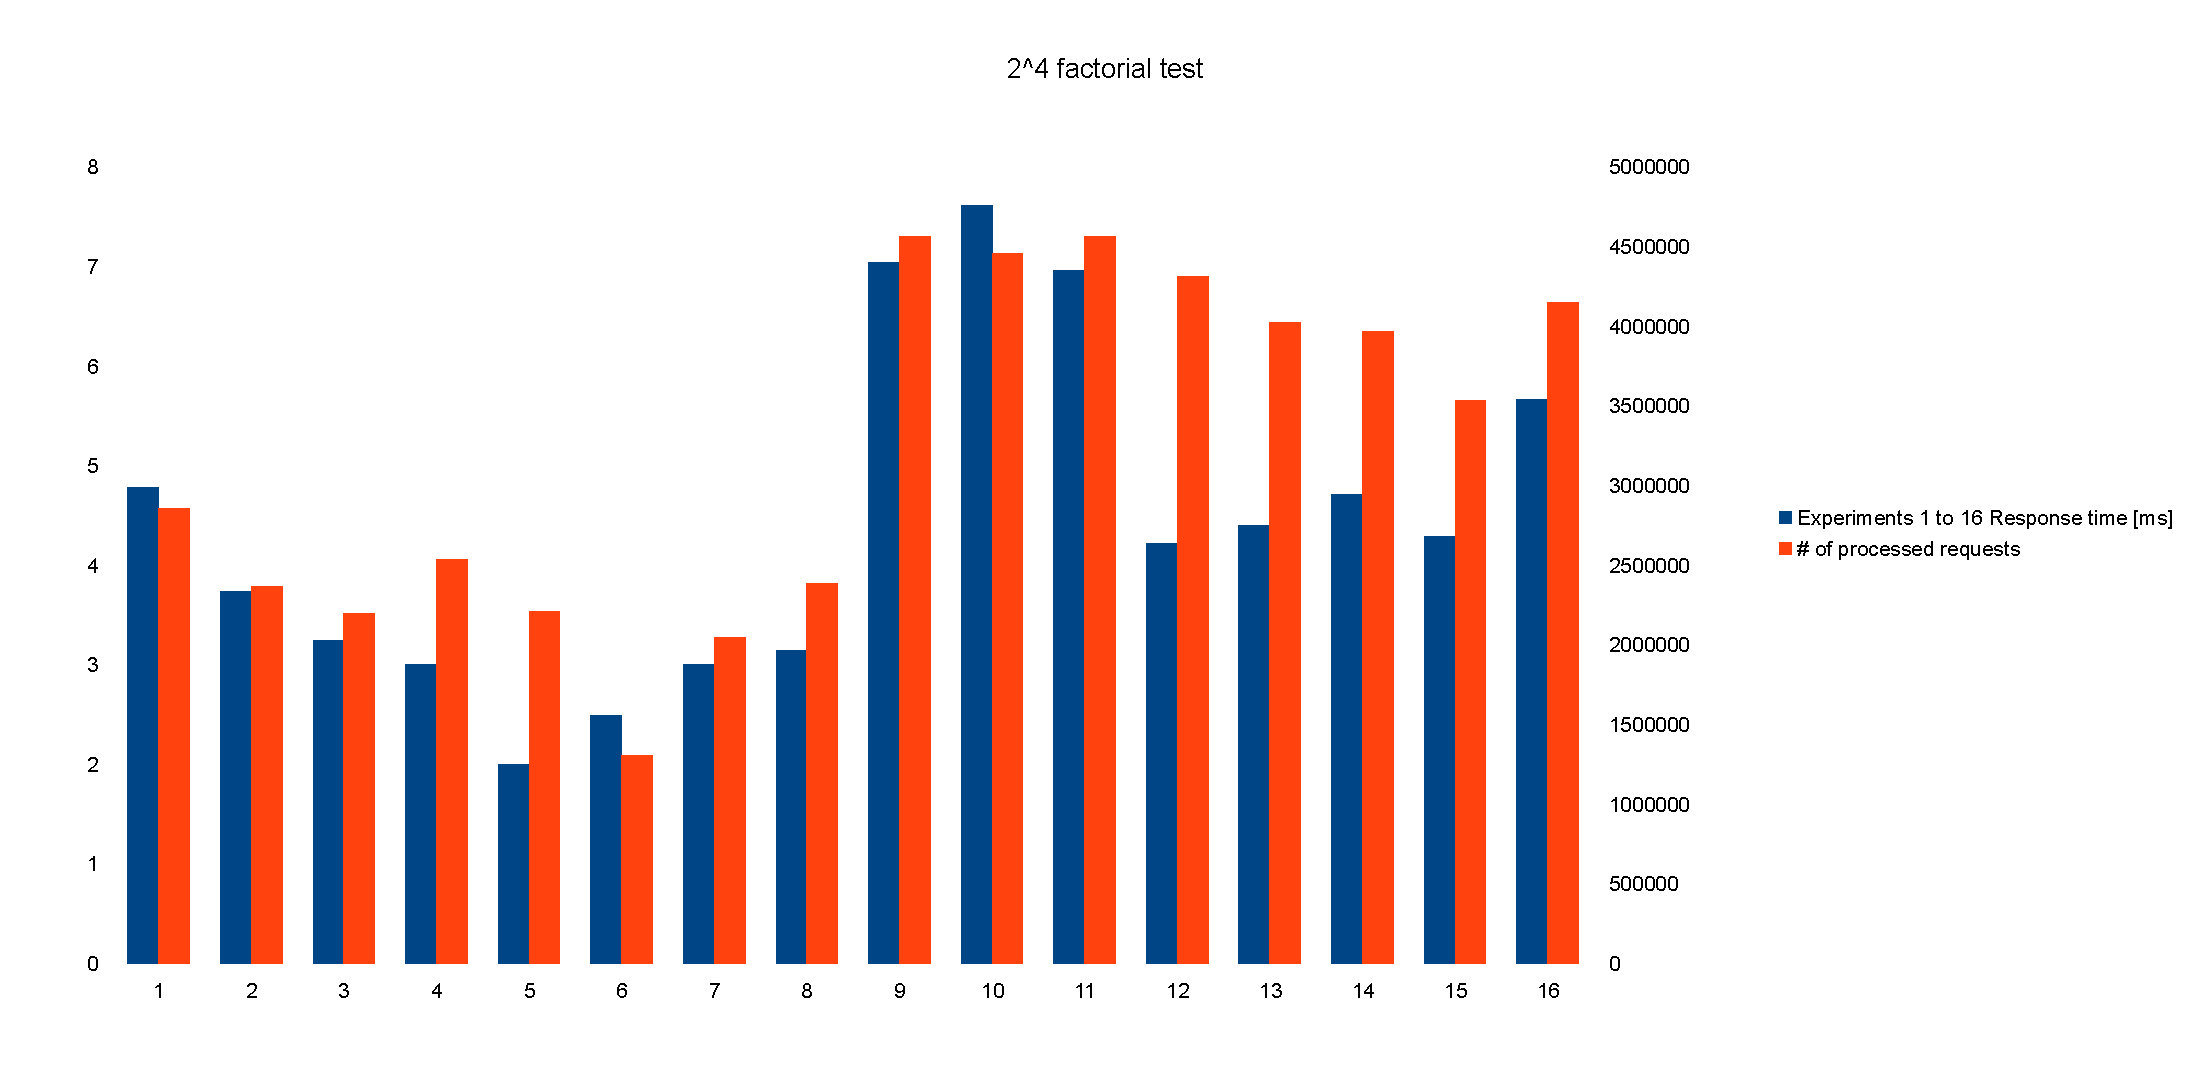
\includegraphics[scale=0.3]{../drawings/2k-factorial-plot.eps}
  \end{center}
  \caption{$2^4$ factorial measured results}
  \label{fig:2kmeasuredresults}
\end{figure}



Mean performance concerning response time has a value of $10.24$. The effect of varying number of clients from 15 to 30 has a weight of $3.43$. This means when increasing the number of clients (and number of requests) the response time also increases. The other values are relatively low. Number of database connections $d$ and number of brokers $b$ in combination with number of database connections  are the next values worth to have a look at. This means that the number of database connections has the most significant impact on response time. By varying number of brokers the total number of database connections also change.

Overall the most significant factor which affects performance the most (beside the load applied by clients) is the number of database connections. This indicates that the database is a bottle neck.

%% -------------------------------------------
\subsection{Db Load Test}

testrun 87 shows what happens when we add more messages than we delete. 

After 2h the database contains 170000 messages
show plots for query peek time, etc
db access gets slower


\subsection{Performance Breakup for Different Tiers}

TODO: db vs client (vs broker?) for load test


\subsection{divers}

testrun 105 - out of disk space

\end{document}